\documentclass[a4paper, 11pt]{article}


\usepackage{amsmath}
\usepackage[cmintegrals]{newtxmath}
\usepackage{bm}
\usepackage{cite}
\usepackage{algorithmic}
\usepackage{graphicx}
\usepackage{xcolor}
\usepackage{url}
\usepackage{epigraph}
\usepackage{caption}
\usepackage{threeparttable}
\usepackage{siunitx}
\usepackage[margin=1.1in]{geometry}
\usepackage{wrapfig}
\newcommand{\lang}{\begin{picture}(5,7)
\put(1.1,2.5){\rotatebox{45}{\line(1,0){6.0}}}
\put(1.1,2.5){\rotatebox{315}{\line(1,0){6.0}}}
\end{picture}}
\newcommand{\rang}{\begin{picture}(5,7)
\put(.1,2.5){\rotatebox{135}{\line(1,0){6.0}}}
\put(.1,2.5){\rotatebox{225}{\line(1,0){6.0}}}
\end{picture}}


\begin{document}


\title{Swipe Without Age and Gender - A React Native Application}

\author{
Aden Kenny - 300334300
}

\maketitle

\section{Program Architecture}

\begin{wrapfigure}{r}{0.5\textwidth}
\centering
\captionsetup{format=hang}
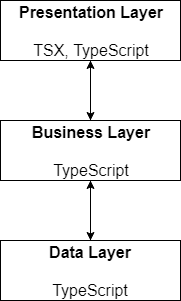
\includegraphics{architecture.png}
\caption{A diagram of the application architecture}
\end{wrapfigure}

Our application has a standard three tier architecture. It has a presentation layer (TSX, and TypeScript), a business layer (TypeScript), and finally a data layer (TypeScript). There is a strict barrier between the three different layers. The data layer can only interact with the business layer, the presentation layer can only interact with the business layer, and the business layer can interact with both the data layer and the business layer. This means that all interactions with external components (database) must go through an intermediary (the business layer) before interacting with the with the user (the presentation layer) or vice versa.

~\\
The presentation layer is the only layer that users will interact with or see. This layer handles all user interaction, and the users should only ever see this layer. This layer, as we used using React Native, is done entirely in TypeScript with TSX. It communicates only with the presentation layer, and is not allowed to interact with the data layer. When communicating with the presentation layer it either sends information about options the user has selected or actions they have carried out. When receiving data from the business layer, the data is related to options or queries the user has made, and this data is then used to update the presentation layer or view that the user sees and provides interactivity between the user and the app.

~\\
The business layer acts as a middleman or glue between the presentation and data layers. The business layer exists exclusively of TypeScript code with functions to parse data from the data layer, functions to update the presentation layer, and functions to modify the state of the system as a whole. All interaction between the presentation layer and data layer must go through the business layer. The overall design means that when the user performs an action such as viewing another users profile, a message will be sent from the presentation layer to the data layer. The business layer will then update, and send a message to the presentation layer to update with some sort of loading behaviour, and a message is then sent to the data layer to fetch the required data to fully update the presentation layer. This data from the data layer is then sent to the business layer where it is parsed for use, and then finally a message is sent to the presentation layer to update to the final state required for the user action.

~\\
The data layer sends data to and from the external Firebase services (see the section 2 below). When fetching data, a message is sent from the business layer to the data layer instructing it to fetch data from the external services. This data is then sent to the business layer. The reverse of this scenario is taken when sending data to the external services (such as sending a message, or updating user details).

~\\
Our architecture matches up pretty well with the standard three-tier model. The presentation and business layers are made up by the files that make up each page, and the data layer is made up by our service class. The presentation layer and business layer are fairly loosely coupled, but due to the fact that React Native forces business and presentation code in the same file, there is definitely some degree of coupling. It would probably require a fairly significant rewrite to change the presentation layer for a different system. The data and business layers are extremely loosely coupled, and the data layer could quite easily be swapped out with another with no adverse consequences.


\section{Firebase Integration}
Our application is a Tinder clone, therefore needs a significant amount of external interaction. We choose to use Firebase for our external storage as it is fairly easily to interact with, and there is good documentation available online. We also have a significant amount of experience with Firebase therefore feel pretty comfortable with using it.

~\\
As our service is account based, the first service we used from Firebase was the authentication service \cite{FirebaseAuth}. This was fairly easy to set up, and it handles all user authentication, from account creation, to logging in. The Firebase authentication service means that users can securely create an account, and their data is safely salted and hashed server side.

~\\
In our application each user has a profile picture, and in order to display this profile picture to other users the picture had to be stored server side. In order to solve this problem we used Firebase Storage. This allowed us to create a folder for each user where their profile picture is saved. When a user views the profile of another user, the profile picture of the second user is downloaded from our Firebase Storage.

~\\
Finally, we used Firebase's Realtime Database \cite{firebaseDB} to store user details, including personal information, and also to store conversations. Getting user details is fairly similar to profile pictures as mentioned above, but since the user data is all text, we can store it in a standard database rather than a specialised file storage solution. Conversations are also stored as text in the database, and both users have one conversation object. This means there are no concurrency issues, and there is a single source of truth without having server-side code.

~\\
In order to integrate our Firebase services into our app, we have a joint database and authentication service, and a reference to them can be gotten by any pages that need them through static getters. All database and authentication actions are in the data layer and are therefore separate and uncoupled from the business and presentation layers.

~\\
I found Firebase simple and pleasant to use, and the only gripe I had with it was the fact that it only supports a NoSQL database. NoSQL is useful in situations where you need to scale your database when you have large amounts reads and writes as the database can be distributed over ordinary, cheap servers. In the case of our app, there isn’t much risk of the database needing to be scaled so a relational database probably would have been better for our needs. Additionally, the non-relational structure of a NoSQL database did not provide much of an advantage to us as our user data was fairly structured and uniform.

\section{UX Decisions} 
\begin{wrapfigure}{r}{0.5\textwidth}
\centering
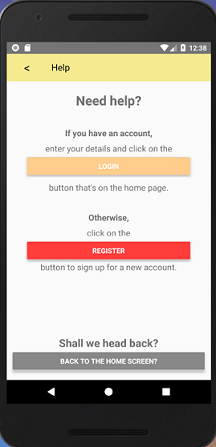
\includegraphics{hierarchy.png}
\caption{A screenshot of the Help page}
\end{wrapfigure}
\subsection{Visual Hierarchy}

The visual hierarchy the order in which a person takes in information in a system, and in the case of a user interface, it is the order in which a person processes information on that specific interface. There are a number of elements which can influence the order in which a user processes the information in terms of UI design \cite{hierarchy}.

\begin{itemize}
	\item{Size}
	\item{Colour}
	\item{Contrast}
	\item{Whitespace}
\end{itemize}

In our app we focused mainly on using size, colour, and whitespace for establishing a clear visual hierarchy. Larger elements were specifically designed this way as they were where we wanted to draw a user's attention to first. A bright red colour was used when we wanted to draw a user's attention to an important button (Register, send a message), and the bright colour would contrast against the white background, which drew the user's attention even more. Whitespace was also used, as the more whitespace around an element, the more a user's attention is drawn to it. Elements that we wanted to draw attention to were given a significant amount of padding, which helped to distinguish them from the rest of the user interface.

~\\
The Help page is a good example of these techniques being used. When a user has clicked on the help page, they are clearly confused and need help with using the app. This means that we want to strongly guide them on this specific page. Therefore we use some of the techniques discussed above to guide the user to where they need to be on the page. First of all, we use a large font for the "Need help?" line, and this is the largest element on the page which, along with being at the top of the page, means that a user will be drawn towards it when they first view the page. The next thing a user will see is the bright red register button, which is clearly marked "REGISTER", and if a user knows they want to sign up for an account, they're likely to click on it. This combination of visual hierarchy techniques mean that a user's attention is drawn to the elements that we want them to use, which are the ones that will hopefully help the user the most.

\subsubsection{Alternative - A Horizontal Visual Hierarchy}
An alternative design decision could have been to create a different, more horizontal visual hierarchy. Currently our visual hierarchy is very horizontally focused. This makes sense for the development of an app that is mainly designed for phones in portrait view, but it may prove to be a poor design decision if a user was using the app on a tablet or a phone in landscape view. 

~\\
A more horizontal visual hierarchy would probably take advantage of a English speaker's instinct to read from left to right, whereas a vertical visual hierarchy would take advantage of a user's propensity to view things from top to bottom.

~\\
Overall a horizontal visual hierarchy would probably be rather unfamiliar to our users, which would hurt the user experience of our app (see Section 3.2 - Jakob's Law). Additionally, in most use cases (a phone in portrait view), a horizontal visual hierarchy would probably not work as well as a vertical visual hierarchy.


\begin{figure}
\centering
\begin{minipage}{.55\textwidth}
  \centering
  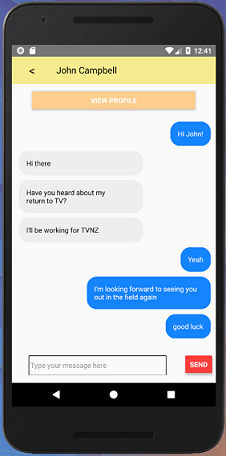
\includegraphics[width=.7\linewidth]{messenger.png}
  \captionof{figure}{A screenshot of the Home page showing the alternate, cool colour palette}
  \label{fig:test1}
\end{minipage}%
\begin{minipage}{.55\textwidth}
  \centering
\captionsetup{format=hang}
  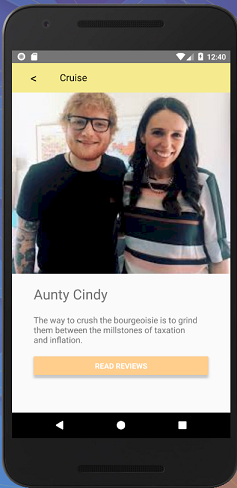
\includegraphics[width=.7\linewidth]{cindy.png}
  \caption{A screenshot of the Hub page}
  \label{fig:test2}
\end{minipage}
\end{figure}
\subsection{Jakob's Law}

Jakob's Law states that "Users spend most of their time on other sites. This means that users prefer your site to work the same way as all the other sites they already know." \cite{jakobs}. A user will be more comfortable using a user interface if it is visually and functionally similar to a user interface they are already familiar with. The user will also probably be more efficient while using a familiar interface. This means that without a good reason to not, you should always try to make your user interface work in a similar way to user interfaces of popular programs.



~\\
We have taken this design principle to heart in most of the pages in our app. The apps that we felt were most similar to ours, and therefore where we would draw inspiration from were Tinder and Facebook Messenger. The influence of Facebook Messenger can clearly be seen a screenshot of our Conversation page (see Figure 3). The interface should feel familiar to users, due the standard "bubble" messaging interface. Another point of familiarity would be the "chat bar" at the bottom of the screen where a user types in their message.

~\\
Another example of Jakob's Law in our application is in the Cruise screen (see Figure 4). This screenshot shows the cruise screen, the place where the user will swipe left or right on people depending on if they're interested in that person. This will be familiar to many of the users of our app as it is very similar to the interface of Tinder.

\subsubsection{Alternative - Jakob's Law, Again}
An alternative design decision could have been to create a user interface that departs quite significantly from precursor applications such as Tinder and Facebook Messenger. This would have presented quite a few disadvantages with no certain advantages. Firstly, it has been proven that the user interfaces of these apps work as they are both very popular, and one should probably have a very good reason for doing something radically different. Secondly, this project had a limited time frame, and coming up with, and implementing a novel user interface and user experience would have been out of scope for this assignment. Thirdly, and perhaps most importantly, we didn't have a novel idea for a user interface, and it's pretty hard to come up with a new user interface without having an idea, let alone a good one.

\subsection{Strong Calls to Action}

\begin{wrapfigure}{r}{0.5\textwidth}
\centering
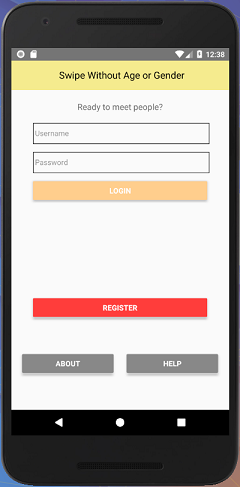
\includegraphics{home.png}
\caption{A screenshot of the Home page}
\end{wrapfigure}

Another major design decision we made during the development of this app was strong calls to action. A call to action is designed to prompt a response from a user, in this case, generally click a button. These calls to action can therefore guide a user to where we want them to be.

~\\
An example of this in our app is on the Home page (see Figure 5). In the screenshot a clear call to action is visible, the Register button. This button is at the top of the visual hierarchy, and it stands out due to a combination of the whitespace around it, and the bright red colour. When a user first gets the the Home page they are either a previous user and probably don't need guidance around the app, or they are new to the app and need strong guidance. The call to action of the Register button will draw the user in to where we want them to go, to the Register page where they can create an account.




\section{React Native Critique}

In this section React Native will be contrasted and compared to Ionic, and React (the web version, which will be referred to as ReactJS for clarity).

~\\
React Native and Ionic are similar as they are both mobile development frameworks that allow the creation of cross platform applications using JavaScript. A major difference between the two is Ionic uses HTML and Sass for creation and styling of the user interface and React Native uses JavaScript, in the form of JSX. React Native's approach of using JavaScript for the application logic and the user interface presents both advantages and disadvantages when contrasted to Ionic which uses HTML and 
Sass for the user interface, or ReactJS which is allows the mixing of HTML, CSS, and JSX.

~\\
JSX is used by both React Native and ReactJS and Facebook, the creators of React Native and ReactJS state the main advantage of their technology, in ReactJS (or React Native), is that "Instead of artificially separating technologies by putting markup and logic in separate files, React separates concerns with loosely coupled units called “components” that contain both." \cite{advantages}. The usage of JSX in React Native means that there is no HTML or CSS used. Instead the user interface and styling of the user interface are defined in the same JavaScript file where the application logic is contained. Facebook therefore seems to think that a major disadvantage of normal web or non-native web development is the usual three file system of HTML, CSS, and JavaScript. They refer to this as "artificially separating technologies", but it is fairly clear that it is a good idea to separate the user interface as a whole from the application logic \cite{sep}, and the React team's argument that a standard separation of concerns is "artificial" is frankly laughable as it can, quite easily, be argued that having items in the same file/class means that they are not truly separated.

~\\
In ReactJS (the web version) the usage of JSX is optional, and I feel that this is a good compromise when compared to React Native that forces the usage of only JSX. Additionally, in ReactJS, a programmer can use standard HTML elements (e.g. \lang  div\rang, \lang li\rang,  \lang b \rang, etc.) but in React Native, a programmer cannot use standard HTML elements as HTML is not supported (without a significant amount of effort and third party libraries). This means that a programmer will find it difficult to simple tasks in React Native that would be trivial in a situation when HTML could be used. For a good example of this is is trying to show a list of bullet points, in HTML it is as simple as using \lang li \rang and \lang ul \rang tags. In React Native you'd either have to deal with a FlatList and all the added complexity that comes with that, or use a ListView and use the unicode character for a bullet point at the start of each line \cite{bullet}, which is quite frankly absurd. I think the ideal scenario for React Native would be to allow the mixing of React components, and HTML elements, as it allows the programmer to have a choice rather than being railroaded into a situation which may prove to make their job more complex, which is the exact opposite of what you want out of a framework/language.

~\\
Another major design decision made by the developers of  React Native is the usage of their own stylesheets rather than the usage of CSS. They state that one of the advantages of this is the fact that this means all styling is in JavaScript rather than having to worry about knowing and using another language (CSS). Unfortunately, React Native's stylesheets just feel like cheap ripoffs of CSS, rather impressively, they manage to incorporate the (many) bad parts of CSS with none of the (few) good parts. The fact that React Native doesn't use CSS means that any CSS orientated tooling such as CSS superscripts (Sass, PostCSS) or even simple IDE features like autocomplete are useless to the developer. Documentation of React Native's stylesheets is also poor, especially relative to CSS, which has a massive amount of information out there. Overall React Native's stylesheets present no appreciable advantages over CSS, but present many disadvantages as they are quite new compared to CSS and haven't had the time to mature. Additionally, ReactJS allows the use of CSS for styling which makes using ReactJS a much more pleasant development experience when compared to React Native.

~\\
One of the biggest issues with React Native is any previous HTML and CSS knowledge is rendered obsolete due to React Native's focus on faux-HTML and faux-CSS. Any developer coming in React Native is likely to have HTML and CSS knowledge, and with the way React Native forces you to use user interfaces, this previous knowledge isn't particularly useful. Facebook presents this as an advantage as they say that you only have to know one language rather than three, but HTML and CSS aren't the most complex languages, and are fairly easy to learn, so I feel that this point falls a little flat.

~\\
My biggest personal gripe is the fact that when creating an Android version of a React Native application, you feel like you're not getting the same experience as you would if you were targeting iOS. There are numerous bugs that we found over the course of development that were due to React Native, and they were Android specific. Quite frequently you would see that the bug had been raised as an issue a significant length of time ago, and the issue was either ignored by the React Native developers or they'd stated that it wasn't a priority to fix as. This is in contrast to any iOS bugs which were quickly fixed.

~\\
Ionic feels like a suitable alternative to native (Android, iOS) development as it provides a completely different development experience when compared to native development, whereas React Native just feels off. Little things that were simple in Ionic, like unordered lists, were far more difficult than they should have been in React Native. Overall, if I wanted to develop a cross-platform app in the future I'd use Ionic, and if I wanted to do something more more I'd just an Android app and an iOS app. React component architecture works well in ReactJS when it can be mixed with HTML and CSS, but it really falls flat in React Native.

~\\
Overall, I find React Native to be extremely impressive, not because it's actually good, but because it makes me miss Ionic, HTML, and CSS. This is a major triumph of mankind, and puts it in the running for the eighth wonder of the world.

\section{Appendices}
\subsection{Division of Work}
For this project I worked in a pair with Simon Pope (3003343009). The app idea and architecture are a joint work, and then we divided the pages between us and then worked on them separately.

\subsubsection{Joint Work}
\begin{itemize}
	\item{Architectural Design}
	\item{Data services (entire data layer)}
\end{itemize}

\subsubsection{Aden}

\begin{itemize}
	\item{About Page}
	\item{Conversation Page}
	\item{Help Page}
	\item{Home Page}
	\item{Loading Page}
	\item{Message Hub Page}
	\item{Register Page}
\end{itemize}

\subsubsection{Simon}

\begin{itemize}
	\item{Cruise Page}
	\item{Edit Details Page}
	\item{Hub Page}
	\item{Match Page}
	\item{Post Review Page}
	\item{Review Page}
	\item{View Match Page}
	\item{View Profile Page}
\end{itemize}

\bibliographystyle{ieeetr}

\bibliography{bibliography}
\end{document}